\graphicspath{{../../S18_Le_ratio/Images/}}

\themeO
\chapter{Le ratio}
\label{S18}

\programme%
   {\item Notion de ratio.}
   {\item Partager une quantité (par exemple une somme d’argent) en deux ou trois parts selon un ratio donné.}

\vfill

\begin{debat}{Débat : d'où vient le ratio ?}
   {\bf Ratio} vient de l’anglais {\bf ratio} que l’on traduit par proportion qui lui-même vient du latin {\bf ratio} qui signifie calcul ou compte. Ce vocabulaire est plutôt utilisé dans le monde anglo-saxon. \par
   On le retrouve pour la première fois dans {\it Les éléments}, d'{\it Euclide}, soit il y a environ 2\,300 ans !
   \tcblower
      \begin{pspicture}(0,0)(7.5,4.7)
      {\psset{unit=0.35}
         \psgrid[subgriddiv=0,gridcolor=lightgray,gridlabels=0pt](0,0)(21,13)
         \psframe(0,0)(21,13)
         \psline(8,0)(8,13)
         \psline(0,8)(8,8)
         \psline(5,8)(5,13)
         \psline(5,10)(8,10)
         \psline(6,8)(6,10)
         \psline(5,9)(6,9)
         \psset{linecolor=DarkViolet,linewidth=0.2}
         \psarc(8,13){13}{-90}{0}
         \psarc(8,8){8}{180}{-90}
         \psarc(5,8){5}{90}{180}
         \psarc(5,10){3}{0}{90}
         \psarc(6,10){2}{-90}{0}
         \psarc(6,9){1}{90}{-90}}
      \end{pspicture}
\end{debat}

\hfill {\gray Vidéo : \href{https://www.youtube.com/watch?v=vDZje8o_eD4}{\bf Quel est le point commun entre un ananas, des lapins et la tour de Pise ?}, chaîne {\it Unisciel}.}


%%% Approche %%%
\begin{Maquette}[Cours]{Theme={Activité d'approche},Couleur={SteelBlue}}

   \AAtitre{Représenter des ratios}

      {\it Objectifs : calculer un ratio ; partager une quantité en deux ou trois parts selon un ratio donné.}

      \begin{AActivite}

         \begin{minipage}{7cm}
            {\psset{unit=0.8}
            \begin{pspicture}(-0.5,-0.5)(8,3.7)
               \psline(0,3)(0,0)(8,0)(8,3)
               \pscircle(1,0.5){0.5}
               \pscircle[fillstyle=solid,fillcolor=lightgray](2,0.5){0.5}
               \pscircle[fillstyle=solid,fillcolor=lightgray](3,0.5){0.5}
               \pscircle(4.5,0.5){0.5}
               \pscircle(5.5,0.5){0.5}
               \pscircle[fillstyle=solid,fillcolor=black](7,0.5){0.5}
               \pscircle(0.5,1.4){0.5}
               \pscircle[fillstyle=solid,fillcolor=lightgray](1.5,1.4){0.5}
               \pscircle(2.5,1.4){0.5}
               \pscircle(3.75,1.2){0.5}
               \pscircle[fillstyle=solid,fillcolor=black](5,1.4){0.5}
               \pscircle[fillstyle=solid,fillcolor=lightgray](6.25,1.2){0.5}
               \pscircle(7.5,1.4){0.5}
               \pscircle[fillstyle=solid,fillcolor=black](2,2.3){0.5}
               \pscircle(3.25,2.1){0.5}
               \pscircle[fillstyle=solid,fillcolor=lightgray](4.25,2.1){0.5}
               \pscircle(5.75,2.1){0.5}
               \pscircle(6.75,2.1){0.5}
               \pscircle[fillstyle=solid,fillcolor=black](5,2.8){0.5}
               \pscircle[fillstyle=solid,fillcolor=lightgray](3.75,3){0.5}
            \end{pspicture}}
         \end{minipage}
         \quad
         \begin{minipage}{9cm}
            Dans cette boite, il y a 4 balles noires pour 6 balles grises. \par
            On dit que la quantité de balles noires et grises est dans le ratio de 4 : 6 (on lit \og 4 pour 6 \fg{}) ou encore 2 : 3 (\og 2 pour 3 \fg{}). \par
         Inversement, le ratio des balles grises et noires est de 6 : 4.
         \end{minipage}
         \begin{enumerate}
            \item 
               \begin{enumerate}
                  \item Quel est le ratio des balles noires et blanches ? Simplifier éventuellement ce ratio. \par \smallskip
                     \pointilles
                  \item Quel est le ratio des balles grises et blanches ? Simplifier éventuellement ce ratio. \par \smallskip
                     \pointilles
                  \item Comment pourrait-on écrire le ratio de balles noires, grises et blanches ? \par \smallskip
                     \pointilles
                  \item Quelle fraction du total des balles représente les balles noires ? Les balles grises ? Les balles blanches ? \par \smallskip
                     \pointilles
               \end{enumerate}
            \item Dans cette question, on garde les mêmes ratios que dans les questions précédentes.
               \begin{enumerate}
                  \item Si le bac contenait 40 balles, combien aurait-on de balles noires ? grises ? blanches ? \par \smallskip
                     \pointilles \par
                     Quelle fraction du total des balles représente chaque sorte de balles ? \par \smallskip
                     \pointilles
                  \item Si le bac contenait 10 balles, combien aurait-on de balles noires ? grises ? blanches ? \par \smallskip
                     \pointilles \par
                     Quelle fraction du total des balles représente chaque sorte de balles ? \par \smallskip
                     \pointilles
                  \item Si le bac contenait 130 balles, combien aurait-on de balles noires ? grises ? blanches ? \par \smallskip
                     \pointilles \par
               Quelle fraction du total des balles représente chaque sorte de balles ? \par \smallskip
                     \pointilles
               \end{enumerate}
            \item On souhaite partager 21 balles roses et violettes dans le ratio 3 : 4. Combien aura-t-on de balles roses et violettes ? \par \smallskip
               \pointilles
           \item On partage 48 balles bleues, blanches et rouges dans le ratio 1 : 2 : 3. Combien a-t-on de balles de chaque couleur ? \par \smallskip
            \pointilles
         \end{enumerate}

      \end{AActivite}

\end{Maquette}


%%%Trace écrite %%%
\begin{Maquette}[Cours]{Theme={Trace écrite},Couleur={0.4[SteelBlue,Black]}}

   %%%1
   \section{Définition du ratio}

      \begin{definition*}{}
         \begin{itemize}
            \item On dit que {\bf deux nombres} $a$ et $b$ sont, par exemple, dans le {\bf ratio} 3 : 4 si $\dfrac{a}{3} =\dfrac{b}{4}$. \par
               On parle de ratio \og trois pour quatre \fg. \par \smallskip
               On peut le modéliser ainsi : \parbox{7cm}{\Ratio[FigureCours,Longueur=7cm,CouleurUn=DodgerBlue,CouleurDeux=Crimson]{3,4}}
            \item On dit que {\bf trois nombres} $a$, $b$ et $c$ sont, par exemple, dans le {\bf ratio} 1 : 3 : 6 si $\dfrac{a}{1} =\dfrac{b}{3} = \dfrac{c}{6}$. \par
               On parle de ratio \og un pour trois pour six \fg. \par \smallskip
               On peut le modéliser ainsi : \parbox{7cm}{\Ratio[FigureCours,Longueur=8cm,CouleurUn=DodgerBlue,CouleurDeux=Crimson,CouleurTrois=Gold]{1,3,6}}
         \end{itemize}
      \end{definition*}

      \begin{exemple*}{}
         Sara et Nathanael se partagent des cookies dans un ratio 3 : 4, cela veut dire que, à chaque fois que Sara a 3 cookies, Nathanael en a 4 si bien que le nombre de cookies que possède Sara divisé par 3 est toujours égal au nombre de cookies que possède Nathanael divisé par 4.
      \end{exemple*}

      Remarque : attention à ne pas confondre les notations 3 : 4 ; $3\div4$ et $\dfrac34$, la première désigne un ratio, la deuxième une division et la troisième une fraction. \par
         Dans l'exemple, Sara possède $\dfrac37$ des cookies et Nathanael $\dfrac47$. \par \smallskip
         Chacune de ces fractions permet de comparer une partie à la totalité, ce ne sont pas des ratios.


   %%%2
   \section{Méthode de partage suivant un ratio}

      \begin{methode*}{Partager suivant un ratio}
         Pour partager une quantité suivant un ratio :
         \begin{enumerate}
            \item on calcule le nombre de parts égales à distribuer en additionnant les nombres du ratio ;
            \item on divise la quantité par le nombre de parts à distribuer ce qui nous donne la quantité par part ;
            \item on distribue les parts selon le ratio.
         \end{enumerate}
         \begin{exbmethode}
            On souhaite partager 15 pièces d'or entre les deux pirates Sambra et Piébo suivant le ratio 2 : 3. \par
            Combien vont-ils avoir de pièces d'or chacun ?
            \tcblower
               \begin{itemize}
                  \item Les 15 pièces d'or sont partagées en 5 parts égales (2 parts pour Sambra et 3 parts pour Piébo).
                  \item $15\text{ pièces d'or}\div 5 =3\text{ pièces d'or}$ donc, une part vaut 3 pièces d'or.
                  \item Sambra a 2 parts, soit $2\times3\text{ pièces d'or} =6\text{ pièces d'or}$ \par
                     Piébo a 3 parts, soit $3\times3\text{ pièces d'or} =9\text{ pièces d'or}$. 
               \end{itemize}
            \end{exbmethode}
      \end{methode*}

      \begin{center}
         \Ratio[Figure,TexteTotal=15 pièces,Longueur=12cm,CouleurUn=DodgerBlue,CouleurDeux=Crimson]{2,3}
      \end{center}

\end{Maquette}


%%% Exercices %%%
\begin{Maquette}[Fiche,CorrigeFin,Colonnes=2]{}
   
   \begin{multicols}{2}

      \begin{exercice} %1
         Simplifier les ratios suivants.
         \begin{colenumerate}[3]
            \item 35 : 20
            \item 49 : 70
            \item 18 : 24
         \end{colenumerate}
      \end{exercice}
      
      \begin{Solution}
         \begin{colenumerate}[3]
            \item \cor{7 : 4}
            \item \cor{7 : 10}
            \item \cor{3 : 4}
         \end{colenumerate}
      \end{Solution}
      
      
      \begin{exercice} %2
         Ratios et bonbons.
         \begin{enumerate}
            \item Un paquet de bonbons contient 13 bonbons à la fraise et 8 au citron. Dans quel ratio sont les bonbons à la fraise et les bonbons au citron ?
            \item Un paquet de bonbons contient 28 bonbons à la fraise, 18 au citron et 14 au cola. Dans quel ratio sont les bonbons à la fraise, les bonbons au citron et les bonbons au cola ?
         \end{enumerate}
      \end{exercice}
      
      \begin{Solution}
         \begin{enumerate}
            \item Les bonbons à la fraise et au citron sont dans le ratio \cor{13 : 8}
            \item Les bonbons à la fraise, au citron et au cola sont dans le ratio \cor{28 : 18 : 14} ou encore 14 : 9 : 7
         \end{enumerate}
      \end{Solution}
      
      
      \begin{exercice} %3
         Utiliser le dessin ci-dessous pour répondre aux questions.
         \begin{center}
         \psset{unit=0.7,subgriddiv=0,gridlabels=0,fillstyle=solid}
            \begin{pspicture}(0,0)(7,2.5)
               \def\noir{\psframe[fillcolor=black](0,0)(1,1)}
               \rput(0,0){\noir}
               \rput(0,2){\noir}
               \rput(3,0){\noir}
               \rput(3,2){\noir}
               \rput(6,0){\noir}
               \rput(6,2){\noir}
               \psframe[fillcolor=lightgray](1,1)(3,2)
               \psframe[fillcolor=lightgray](4,1)(6,2)
               \psgrid(0,0)(7,3)
            \end{pspicture}
         \end{center}
         \begin{enumerate}
            \item Quel est le ratio carrés gris - total de carré ?
            \item Que peut représenter le ratio 4 : 6 ?
            \item Selon quel ratio sont représentés les carrés noirs et les carrés blancs ?
         \end{enumerate}
      \end{exercice}
      
      \begin{Solution} 
         \begin{enumerate}
            \item Le ratio carrés gris - total de carré est \cor{4 : 21}
            \item 4 : 6 représente le \cor{ratio des carrés gris et des carrés noirs.}
            \item Les carrés noirs et les carrés blancs sont dans le ratio \cor{6 : 11}
         \end{enumerate}
      \end{Solution}
      
      
      \begin{exercice} %4
         Utiliser ce tableau des matchs perdus ou gagnés d'un collège pour répondre aux questions.
         \begin{center}
            {\hautab{1.2}
            \begin{tabular}{|*4{C{1.8}|}}
               \hline
               & matchs gagnés & matchs perdus \\
               \hline
               Rugby & \quad\, 9 & \quad\, 6 \\
               \hline
               Judo & \quad 12 & \quad\, 8 \\
               \hline
               Handball & \quad 10 & \quad\, 5 \\
               \hline
            \end{tabular}}
         \end{center}
         \begin{enumerate}
            \item Quels sports ont un ratio équivalent gains-pertes ?
            \item Pour le handball :
            \begin{enumerate}
               \item Quel est le ratio gains-matchs joués ?
               \item Quelle est la fraction de matchs gagnés ?
            \end{enumerate}
         \end{enumerate}
      \end{exercice}
      
      \begin{Solution}
        \begin{enumerate}
            \item Ratio gains-pertes : Rugby 9 : 6 $=$ 3 : 2 ; Judo 12 : 8 $=$ 3 : 2 ; Handball 10 : 5 $=$ 2 : 1. \cor{Le rugby et le judo ont même ratio.}
            \item 
               \begin{enumerate}
                  \item Ratio gains - matchs joués : 10 : 15 équivalent à \cor{2 : 3} \par
                  \item Fraction de matchs gagnés : $\dfrac{10}{15} =\cor{\dfrac23}$ \par
               \end{enumerate}
         \end{enumerate}
      \end{Solution}
      

      \begin{exercice} %5
         Dans une assemblée, le ratio hommes-femmes est de 50 : 45. \par
         Si cinq femmes entrent, le ratio sera-t-il de 50 : 50 ?
      \end{exercice}
      
      \begin{Solution}
         Un ratio hommes-femmes de 50 : 45 signifie qu'il y a 50 hommes pour 45 femmes. Dans une assemblée de 500 hommes et 450 femmes, si 5 femmes entrent on aura 500 hommes pour 455 femmes soit \cor{un ratio de 500 : 455}.
      \end{Solution}


      \begin{exercice} %6
         Des ratios \og doubles \fg.
            \begin{enumerate}
               \item Quelle quantité d'huile et de vinaigre utilise-t-on dans une vinaigrette de \Capa{500} réalisée dans le ratio 3~:~1 ?
               \item Deux amis ont joué au loto et leur mise s'est faite selon le ratio 3 : 5. Ils gagnent \Prix{64}. Quelle est la somme d'argent qui revient à chacun d'eux ?
         \end{enumerate}
      \end{exercice}
      
      \begin{Solution}
         \begin{enumerate}
            \item Le ratio 3 : 1 pour l'huile est le vinaigre signifie que pour 3 parts d'huile, on a 1 part de vinaigre pour un total de 4 parts de vinaigrette correspondant à une capacité de \Capa{500}. \par
               \qquad \Ratio[Figure,Longueur=6cm,TexteTotal=\Capa{500},CouleurUn=DodgerBlue,CouleurDeux=IndianRed]{3,1} \par
               $500\div4 =125$ donc, une part vaut \Capa{125}. \par
               Il faut \cor{\Capa{375} d'huile pour \Capa{125} de vinaigre.}        
            \item Le ratio 3 : 5 signifie que pour 3 parts pour le premier ami, le second gagne 5 parts pour un total de 8 parts, correspondant à une somme de \Prix{64}. \par
               %\qquad \Ratio[Figure,Longueur=6cm,TexteTotal=\Prix{64},CouleurUn=DodgerBlue,CouleurDeux=IndianRed]{3,5} \par
               $64\div8 =8$ donc, une part vaut \Prix{8}. \par
               \cor{Le premier ami gagnera \Prix{24} et l'autre \Prix{40}.}
         \end{enumerate}
      \end{Solution}
      

      \begin{exercice} %7
         Des ratios \og triples \fg.
         \begin{enumerate}
            \item Une recette de biscuits sablés commence par la fabrication d'un \og sable \fg{} réalisé avec de la farine, du beurre et du sucre dans le ratio 10 : 6 : 5. Une pâte homogène est ensuite fabriquée avec ce sable et un peu de lait. \par
               Quelles masses de farine, de beurre et de sucre doit-on prendre pour créer un \og sable \fg{} de \Masse{630} ?
            \item Pour récompenser leurs enfants Clémentine, Myrtille et Prune, qui les ont beaucoup aidés, M. et Mme Potager leur donnent un peu d'argent. Ils leur distribuent \Prix{120} selon le ratio 3 : 4 : 5 parce qu'ils n'ont pas aidé autant les uns que les autres. \par
               Combien chacun va-t-il recevoir ?
         \end{enumerate}
      \end{exercice}
      
      \begin{Solution}
         \begin{enumerate}
            \item Le ratio 10 : 6 : 5 pour la farine, le beurre et le sucre signifie que pour 10 parts de farine, on a 6 parts de beurre et 5 parts de sucre pour un total de 21 parts de \Masse{630}. \par
               \qquad \Ratio[Figure,Longueur=7cm,TexteTotal=\Masse{630},CouleurUn=DodgerBlue,CouleurDeux=IndianRed,CouleurTrois=Gold]{10,6,5} \par
               $630\div21 =30$ donc, une part vaut \Masse{30}. \par
               Il faut \cor{\Masse{300} de farine, \Masse{180} de beurre et \Masse{150} de sucre.}
            \item Le ratio 3 : 4 : 5 pour Clémentine, Myrtille et Prune signifie que pour 3 parts pour Clémentine, on a 4 parts pour Myrtille et 5 parts pour Prune pour 12 parts à \Prix{120}. \par
               %\quad \Ratio[Figure,Longueur=7cm,TexteTotal=\Prix{120},CouleurUn=DodgerBlue,CouleurDeux=IndianRed,CouleurTrois=Gold]{3,4,5} \par
               $120\div12 =10$ donc, une part vaut \Prix{10}. \par
               \cor{Clémentine reçoit \Prix{30}, Myrtille \Prix{40} et Prune \Prix{50}.}
         \end{enumerate}
      \end{Solution}
      
      
      \begin{exercice}[Dur] %8
         Les macarons.
         \begin{enumerate}
            \item Comment partager 48 macarons entre Yasmine et Juliette dans le ratio 5 : 11 ?
            \item Yasmine, Juliette et Antoine se partagent des macarons dans le ratio 4 : 3 : 2. Juliette en a 9, combien en ont Kawtar et Talita ?
            \item Juliette et Antoine ont réalisé un certain nombre de macarons dans le ratio 5 : 8. Sachant qu'Antoine, plus expérimentée, a fait 66 macarons de plus que Juliette, combien Antoine en a préparé ?
         \end{enumerate}
      \end{exercice}
      
      \begin{Solution}
         \begin{enumerate}
            \item Le ratio 5 : 11 pour Yasmine et Juliette signifie que pour 5 parts pour Yasmine, Juliette a 11 parts pour un total de 16 parts (48 macarons). \par
               %\qquad \Ratio[Figure,Longueur=7cm,TexteTotal=48 macarons,CouleurUn=DodgerBlue,CouleurDeux=IndianRed]{5,11} \par
               $48\div16 =3$ donc, une part vaut 3 macarons. \par
               \cor{Yasmine aura 15 macarons et Juliette en aura 33.} 
            \item Le ratio 4 : 3 : 2 pour Yasmine, Juliette et Antoine signifie que pour 4 parts pour Yasmine, on a 3 parts pour Juliette et Antoine en a 2 pour un total de 9 parts. \par
               \qquad \Ratio[Figure,Longueur=7cm,TexteTotal=9 parts,CouleurUn=DodgerBlue,CouleurDeux=IndianRed,CouleurTrois=Gold]{4,3,2} \par
               Juliette a 9 macarons, une part vaut donc 3 macarons. \par
               \cor{Yasmine a donc 12 macarons et Antoine en a 6.} 
            \item Le ratio 5 : 8 pour Juliette et Antoine signifie que pour 5 parts pour Juliette, on a 8 parts pour Antoine, soit 3 parts de plus pour Antoine. \par
               \qquad \Ratio[Figure,Longueur=6cm,TexteTotal=3 parts de plus pour Antoine,CouleurUn=DodgerBlue,CouleurDeux=IndianRed]{5,8} \par
               Antoine a fait 66 macarons de plus que Juliette, donc une part vaut 22 macarons ($66\div3$). \par
               \cor{Antoine a donc préparé 176 macarons.} 
         \end{enumerate}
      \end{Solution}
      
      
      \begin{exercice} %9
         Les triangles.
         \begin{enumerate}
            \item Dans quel ratio sont les trois angles d’un triangle équilatéral ?
            \item Dans quel ratio sont les trois angles d’un triangle rectangle isocèle ?
            \item Quelle est la nature d’un triangle dont les angles sont dans le ratio 1 : 2 : 3 ?
         \end{enumerate}
      \end{exercice}
      
      \begin{Solution}
         \begin{enumerate}
            \item Un triangle équilatéral a trois angles de \ang{60}. Les trois angles sont donc dans un ratio de 60 : 60 : 60, soit \cor{1 : 1 : 1}.
            \item Un triangle rectangle isocèle a trois angles de \ang{90}, \ang{45} et \ang{45}. Il sont donc dans un ratio de 90 : 45 : 45, soit \cor{2 : 1 : 1}.
            \item Le ratio 1 : 2 : 3 pour les angles du triangle signifie que pour 1 part pour le premier angle, on a 2 parts pour le second et 3 parts pour le troisième pour un total de 6 parts, correspondant à \ang{180}. \par
               $180\div6 =30$ donc, la valeur d'une part est de \ang{30}. Le triangle a donc trois angles de \ang{30}, \ang{60} et \ang{90}. \par
               \cor{Le triangle est rectangle.} 
         \end{enumerate}
      \end{Solution}

   \end{multicols}
   \vfill\hfill{\footnotesize D'après \href{https://ent2d.ac-bordeaux.fr/disciplines/mathematiques/les-ratios-au-college/}{\og Les ratios au collège \fg}, académie de Bordeaux et \href{https://eduscol.education.fr/document/13132/download}{\og La résolution de problèmes mathématiques au collège \fg}, MENJS, 2021.}

\end{Maquette}


%%% Récré %%%
\begin{Maquette}[Cours]{Theme={Activité récréative},Couleur={IndianRed}}
    
   \ARtitre{The golden ratio}

      \begin{enumerate}
         \item Among the following rectangles, circle the one you think is the most attractive and well-balanced.
            \begin{center}
               \begin{pspicture}(0,0)(14,5)
                  \psset{fillstyle=solid}
                  \psframe[fillcolor=DarkOrange!50](0,0)(2,2)
                  \rput(1,1){a}
                  \psframe[fillcolor=ForestGreen!50](3,0)(7,2.47)
                  \rput(5,1.235){b}
                  \psframe[fillcolor=DarkViolet!50](8,0)(14,2)
                  \rput(11,1){c}
                  \psframe[fillcolor=Crimson!50](0,3)(4,5)
                  \rput(2,4){d}
                  \psframe[fillcolor=DodgerBlue!50](5,3)(14,4)
                  \rput(9.5,3.5){e}
               \end{pspicture}
            \end{center}
         \item Measure each rectangle's length and width, and compare the ratio of length to width for each rectangle above :
            \begin{center}
               {\small \hautab{1.5}
               \begin{tabular}{|c|*5{C{2}|}}
                  \hline
                  Rectangle & a & b & c & d & e \\
                  \hline
                  Length ($\ell$) in \Lg{} & & & & & \\
                  \hline
                  Width ($w$) in \Lg{} & & & & & \\
                  \hline
                  $\ell\div w $ & & & & & \\
                  \hline
               \end{tabular}}
            \end{center}
         \item Draw a segment \Lg{10} long then make a small mark on it \Lg{6.18} along. \par
            Divide the length of the whole line by the length of the long section just made. \par
            Divide the length of the long section by the length of the short section. What ratios do you get? \par \vskip2cm
         \item Unscramble the words to find out the various names of this ratio.
            \begin{center}
               {\hautab{1.5}
               \begin{tabular}{|p{3cm}p{4cm}|p{3cm}p{4cm}|}
                  \hline
                  TEH & \_ \_ \_ & HET & \_ \_ \_ \\
                  DEOGNL & \_ \_ \_ \_ \_ \_ & NODLEG & \_ \_ \_ \_ \_ \_ \\
                  TAIRO & \_ \_ \_ \_ \_ & NOOPOITRRP & \_ \_ \_ \_ \_ \_ \_ \_ \_ \_ \\
                  \hline
                  ETH & \_ \_ \_ & HTE & \_ \_ \_ \\
                  DIINVE & \_ \_ \_ \_ \_ \_ & DEONLG & \_ \_ \_ \_ \_ \_ \\
                  TINPOORPRO & \_ \_ \_ \_ \_ \_ \_ \_ \_ \_ & NEBRUM & \_ \_ \_ \_ \_ \_ \\
                  \hline
               \end{tabular}}
            \end{center}
         \item This number named golden ratio is $\phi =\dfrac{1+\sqrt5}{2}$. Calculate is value with your calculator : \pointilles
      \end{enumerate}
   
      \bigskip
   
      \begin{minipage}{11cm}
         A golden rectangle has a length to width ratio called the golden ratio, which is approximately 1.618. It is used often in art and architecture. For example, the front of the Parthenon, a temple in Athens, Greece fits into a golden rectangle.
      \end{minipage}
      \qquad
      \begin{minipage}{5cm}
         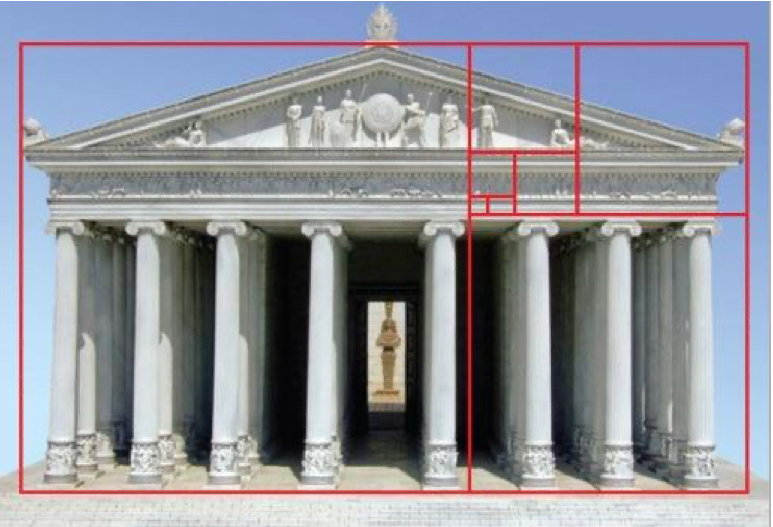
\includegraphics[width=4.5cm]{Parthenon}
      \end{minipage}

\end{Maquette}